\chapter{Mission}
\label{chap:mission}

\section{Overview}
\label{sec:mission_overview}

The \texttt{Mission} class derives from the core \texttt{problem} class and is a top-level container for the entire transcription of an \ac{EMTG} mission. A mission contains a \texttt{boost::ptr\_vector} of \texttt{Journey} objects, each representing one of the mission's journeys. The \texttt{Mission} also holds a \texttt{ObjectiveFunction} object, a vector of \texttt{Universe} objects, and \texttt{Spacecraft} and \texttt{LaunchVehicle} objects. \texttt{Mission} is responsible for the mission flight time constraint as described in Section \ref{sec:mission_time_constraint}, and any propellant or dry mass constraints as described in Section \ref{sec:propellant_and_dry_mass_constraints}.

Each mission contains a vector of \texttt{Journey} objects, each of which contains in turn one or more \texttt{Phase} objects. Each \texttt{Phase} contains a \texttt{DepartureEvent} and an \texttt{ArrivalEvent}. This architecture is flexible and scalable, and describes all of the missions that \ac{EMTG} can optimize as shown in Figure \ref{fig:mission_architecture}

\begin{figure}
	\centering
	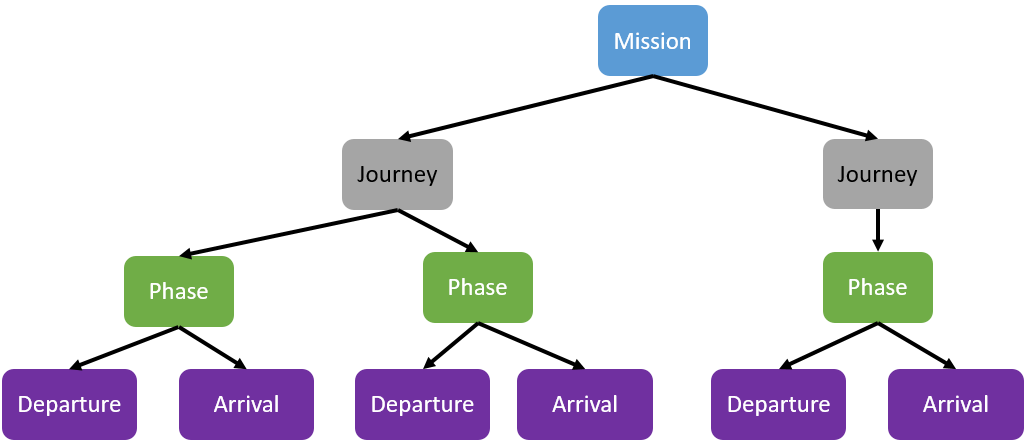
\includegraphics[width=0.9\linewidth]{./mission/EMTG_architecture_diagram.PNG}
	\caption{\label{fig:mission_architecture} Architecture of an \ac{EMTG} mission.}
\end{figure}

The \texttt{Mission} class has the following methods:

\begin{itemize}
	\item \texttt{calcbounds()} - Calculates the upper and lower bounds, as well as scale factors, for any owned decision variables and constraints. Calls the \texttt{calcbounds()} methods of any owned \texttt{Journey} and \texttt{ObjectiveFunction} objects.
	\item \texttt{evaluate()} - Evaluates any owned constraints and their partial derivatives. Calls the \texttt{evaluate()} methods of any owned \texttt{Journey} and \texttt{ObjectiveFunction} objects.
	\item \texttt{output()} - Writes the .emtg output file for the evaluated mission. Calls the \texttt{output()} methods of any owned \texttt{Journey} and \texttt{ObjectiveFunction} objects. Writes the mission-end summary, including all propellant and dry mass information for all spacecraft stages, plus the final decision vector and constraint vector.
	\item \texttt{output\_ephemeris()} - Writes an ephemeris file and acceleration output file for the evaluated mission by calling the \texttt{output\_ephemeris()} of any owned \texttt{Journey} objects. Writes a .cmd and .py file that uses \texttt{mkspk.exe} to create a SPICE kernel from the ephemeris file.
	\item \texttt{output\_STMs()} - Writes text files for each state transition matrix (STM) in the mission by calling the \texttt{output\_STMs()} method on any owned \texttt{Journey} objects.
	\item \texttt{output\_maneuver\_and\_target\_spec()} - Writes maneuver and target specification files by calling the \texttt{output\_maneuver\_and\_target\_spec()} methods of any owned \texttt{Journey} objects. These files are read by PIRATE, MONSTER, PyGMATscripter, and eventually also interfaces to Monte and provide the necessary information to re-target each maneuver in an operational navigation tool.
	\item \texttt{construct\_initial\_guess()} - Constructs the initial guess for the optimization problem. The user-provided \texttt{trialX} field in the \texttt{missionoptions} structure is compared to the mission \texttt{Xdescriptions} vector via string matching. Values from \texttt{trialX} are inserted into the initial guess vector when their descriptions match. If state representations do not match, \textit{i.e.} if the user has specified an initial guess in \texttt{SphericalRADEC} coordinates but the \texttt{missionoptions} file is configured to use \texttt{SphericalAZFPA} coordinates, then the user is warned. Low thrust phase initial guesses, whether they be based on two-point shooting or parallel shooting transcriptions, are interpolated to the number of time segments and interior control points requested by the user for that phase. Once all initial guess values are assigned, they are clipped to remain inside the \texttt{Xupperbounds} and \texttt{Xlowerbounds} vectors that were generated by the constructor. Finally, if any values remain unspecified, \texttt{construct\_initial\_guess} populates the with random values between the allowed bounds.
	\item \texttt{getUnscaledObjective()} - Returns the unscaled value of the objective function.
	\item \texttt{getJourney()} - Returns a pointer to the desired \texttt{Journey} object.
\end{itemize}

In addition, because \texttt{Mission} is \textit{not} derived from \texttt{sparsey\_thing}, \texttt{Mission} also implements the following utility methods:

\begin{enumerate}
	\item \texttt{create\_sparsity\_entry()}
	\item \texttt{create\_sparsity\_vector()}
\end{enumerate}

\section{Mission Time Constraint}
\label{sec:mission_time_constraint}

The user may impose constraint on total mission flight time. This is simply the sum of all of the time variables in the mission. \ac{EMTG} locates these by iterating through the \texttt{Xdescriptions} vector and adding up all decision variables that contain the string ``time.''

\section{Propellant and dry mass constraints}
\label{sec:propellant_and_dry_mass_constraints}

\texttt{Mission} may track constraints on chemical fuel, chemical oxidizer, electric, propellant, and/or dry mass. The user may choose to impose these globally, \textit{i.e.} over the entire mission, or at the spacecraft \texttt{stage} level.

All propellant usage in \ac{EMTG} is tracked by means of ``virtual tank'' variables. The nonlinear computations of true propellant use are book-kept as locally as possible in individual \texttt{Phase} and boundary event objects. Each maneuver is assigned a ``virtual tank'' variable and constraint. The ``virtual tank'' variable is a free parameter and is constrained to match the computed value of actual propellant use. The total amount of each type of propellant may then be computed by a linear sum of all of the associated virtual tank variables.

The \texttt{Spacecraft} object keeps track of the indices in the decision vector corresponding to the virtual tank variables for each propellant type. In addition, each individual \texttt{Stage} object keeps track of the indices corresponding to the virtual tank variables of each propellant type assigned to that stage. \texttt{Mission}'s only responsibility is to sum up all of the virtual tank variables for each global or stage propellant constraint. The lower bound on each propellant tank constraint is 0.0 kg and the upper bound is the user-defined size of the tank, adjusted by the user-defined propellant margin.

The global and stage dry mass constraints are computed by subtracting the total propellant consumed, plus user-defined margin, from the encoded final mass of the spacecraft. If the spacecraft either dropped mass (\textit{e.g.} dropped a probe) or added mass (\textit{e.g.} picked up a rock from an asteroid), then this mass is also accounted for.

Finally, the user may choose to constrain ``final mass'' instead of ``dry mass.'' This is just a constraint applied directly to the final state of the spacecraft, ignoring any propellant margin.